\section{Results}
\label{sec:results}

All Grand Slam results are presented separately for the ATP and WTA tours. Non-Grand-Slam control function results are discussed in Section~\ref{sec:results_nongs} and reported in full in the appendix.

\subsection{Immediate Effects}
\label{sec:results_immediate}

Before examining post-episode dynamics, I characterize the treatment dose---the direct consequences of LL entry at the focal event. Because control players by definition do not enter the main draw, these estimates describe the magnitude of the treatment rather than a causal effect relative to a counterfactual.

Table~\ref{tab:immediate} reports the immediate event-level effects of lottery selection.

On the ATP tour ($N = 248$), 32 percent of treated players win at least one main draw match, earning a median of approximately 35 additional ranking points at the event. Treated players play 1.48 additional matches ($p < 0.001$) and earn 29.66 ranking points on average ($p < 0.001$). The magnitude of the immediate shock is economically meaningful: a Grand Slam first-round loss earns 10 ranking points, while a second-round loss earns 45 points.

On the WTA tour ($N = 132$), 38 percent of treated players win at least one main draw match, play 1.41 additional matches ($p < 0.001$), and earn 24.86 ranking points on average ($p < 0.001$). The smaller WTA point total reflects the different competitive density at the margin.

\begin{table}[htbp]
\centering
\caption{Grand Slam Lottery: Immediate Event-Level Effects}
\label{tab:immediate}
\begin{threeparttable}
\small
\begin{tabular}{l ccc}
\toprule
 & $t$-test & \multicolumn{2}{c}{Event FE} \\
\cmidrule(lr){2-2} \cmidrule(lr){3-4}
Outcome & LL Mean & $\hat{\beta}$ & (SE) \\
\midrule
\multicolumn{4}{l}{\textit{ATP}} \\
\quad Main-draw match win & 0.34$^{***}$ & 0.32$^{***}$ & (0.06) \\
\quad Main-draw matches played & 1.45$^{***}$ & 1.48$^{***}$ & (0.08) \\
\quad Ranking points at event & 28.14$^{***}$ & 29.66$^{***}$ & (3.79) \\
\quad $N$ & \multicolumn{1}{c}{132 / 116} & \multicolumn{2}{c}{248} \\
\addlinespace
\multicolumn{4}{l}{\textit{WTA}} \\
\quad Main-draw match win & 0.39$^{***}$ & 0.38$^{***}$ & (0.06) \\
\quad Main-draw matches played & 1.43$^{***}$ & 1.41$^{***}$ & (0.07) \\
\quad Ranking points at event & 25.28$^{***}$ & 24.86$^{***}$ & (2.71) \\
\quad $N$ & \multicolumn{1}{c}{54 / 78} & \multicolumn{2}{c}{132} \\
\addlinespace
\multicolumn{4}{l}{\textit{Pooled}} \\
\quad Main-draw match win & 0.35$^{***}$ & 0.36$^{***}$ & (0.04) \\
\quad Main-draw matches played & 1.45$^{***}$ & 1.47$^{***}$ & (0.05) \\
\quad Ranking points at event & 27.31$^{***}$ & 28.46$^{***}$ & (2.43) \\
\quad $N$ & \multicolumn{1}{c}{186 / 194} & \multicolumn{2}{c}{380} \\
\bottomrule
\end{tabular}

\begin{tablenotes}
\footnotesize
\item \textit{Notes.} Full Grand Slam sample: top-four ranked final-round qualifying losers at events with at least one LL slot, 2006--2024. ATP: $N = 248$; WTA: $N = 132$. Event FE columns report OLS with Grand Slam $\times$ Year fixed effects. Control outcomes are mechanically zero because unselected players do not enter the main draw. $^{***}p<0.01$, $^{**}p<0.05$, $^{*}p<0.10$.
\end{tablenotes}
\end{threeparttable}
\end{table}

\subsection{Post-Episode Dynamics}
\label{sec:results_dynamics}

Tables~\ref{tab:dynamic_atp} and~\ref{tab:dynamic_wta} report estimates from a stacked specification with horizon-specific treatment effects estimated jointly. The stacked model pools all five horizons into a single regression with horizon-specific LL coefficients and horizon fixed effects, improving efficiency by borrowing information across horizons while allowing the treatment effect to vary freely at each horizon. I present ATP and WTA results separately.

\paragraph{ATP results.} The ATP sample comprises 248 player-episodes contributing approximately 1,200 stacked observations across five horizons. Ranking points increase by 31.9 at 4 weeks ($p = 0.028$), 38.5 at 12 weeks ($p = 0.007$), and 49.2 at 26 weeks ($p = 0.054$). The point gain fades to 4.3 at 52 weeks ($p = 0.919$), consistent with the rolling 52-week window replacing the initial point gain with subsequent results. For reference, the control-group mean ranking point stock is approximately 469 (ATP) and 476 (WTA), so the 26-week gain of 49.2 points represents roughly a 10\% increase relative to baseline. Main draw entries increase by 0.6 at 12 weeks ($p = 0.046$) and 1.1 at 26 weeks ($p = 0.006$); control players enter an average of 4.1 main draws over 26 weeks, so 1.1 additional entries represents a 27\% increase. Matches at 250+ events increase by 0.8 at 12 weeks ($p = 0.110$) and 1.8 at 26 weeks ($p = 0.010$). Elo rating changes are null at every horizon. The pattern confirms that the ranking point boost from the LL event is real but temporary: it builds through 26 weeks as the player enters additional tournaments, then dissipates as the initial points age out of the rolling window.

\paragraph{WTA results.} The WTA sample comprises 132 player-episodes contributing approximately 640 stacked observations. Ranking points increase sharply at 4 weeks (64.4, $p = 0.003$) and 8 weeks (78.7, $p < 0.001$), but the effect dissipates faster than on the ATP tour: the 12-week estimate is 32.3 ($p = 0.135$) and the 26-week estimate is 6.3 ($p = 0.861$), consistent with the WTA's denser tournament calendar accelerating the point cycle. Elo effects are positive at 4 weeks (10.5, $p = 0.070$) and 26 weeks (17.3, $p = 0.072$) but do not reach conventional significance at most horizons. The WTA results should be interpreted with caution given the smaller sample and borderline balance ($p = 0.333$).

\begin{table}[htbp]
\centering
\caption{ATP Grand Slam: Post-Episode Dynamic Effects (Stacked Model)}
\label{tab:dynamic_atp}
\begin{threeparttable}
\small
\begin{tabular}{l*{5}{c}}
\toprule
 & 4w & 8w & 12w & 26w & 52w \\
\midrule
Ranking Pts $\Delta$ & 31.9$^{**}$ & 31.3$^{**}$ & 38.5$^{***}$ & 49.2$^{*}$ & 4.3 \\
 & (14.5) & (14.2) & (14.3) & (25.6) & (42.1) \\[0.3em]
Elo $\Delta$ & -1.6 & 0.2 & -3.9 & 2.8 & -14.5 \\
 & (5.1) & (5.9) & (6.1) & (8.8) & (12.8) \\[0.3em]
Main Draws & 0.2 & 0.5$^{*}$ & 0.6$^{**}$ & 1.1$^{***}$ & 1.3 \\
 & (0.3) & (0.3) & (0.3) & (0.4) & (0.9) \\[0.3em]
Matches 250+ & 0.2 & 0.6 & 0.8 & 1.8$^{***}$ & 2.2 \\
 & (0.6) & (0.5) & (0.5) & (0.7) & (1.8) \\[0.3em]
Win \% & -0.01 & -0.01 & -0.03 & -0.02 & -0.02 \\
 & (0.03) & (0.02) & (0.02) & (0.02) & (0.02) \\[0.3em]
\bottomrule
\end{tabular}

\begin{tablenotes}
\footnotesize
\item \textit{Notes.} Stacked specification: 248 player-episodes contributing 1,200--1,240 stacked observations across five horizons (4, 8, 12, 26, 52 weeks). Horizon-specific LL treatment effects estimated jointly with horizon fixed effects, Grand Slam $\times$ Year fixed effects, and pre-treatment controls (ranking points linear and quadratic, Elo / 100 linear and quadratic, surface Elo / 100 linear and quadratic, prior GS LL spots won, prior GS LL candidacies not won, prior non-GS LL spots won, prior non-GS LL candidacies not won, and age). Standard errors clustered at the player level. $^{***}p<0.01$, $^{**}p<0.05$, $^{*}p<0.10$.
\end{tablenotes}
\end{threeparttable}
\end{table}

\begin{table}[htbp]
\centering
\caption{WTA Grand Slam: Post-Episode Dynamic Effects (Stacked Model)}
\label{tab:dynamic_wta}
\begin{threeparttable}
\small
\begin{tabular}{l*{5}{c}}
\toprule
 & 4w & 8w & 12w & 26w & 52w \\
\midrule
Ranking Pts $\Delta$ & 64.4$^{***}$ & 78.7$^{***}$ & 32.3 & 6.3 & 6.3 \\
 & (21.4) & (22.2) & (21.6) & (36.0) & (66.6) \\[0.3em]
Elo $\Delta$ & 10.5$^{*}$ & 7.4 & 6.5 & 17.3$^{*}$ & 13.4 \\
 & (5.8) & (6.7) & (8.0) & (9.6) & (16.1) \\[0.3em]
Main Draws & 0.1 & 0.5 & 0.5 & 0.8$^{*}$ & 1.2 \\
 & (0.3) & (0.3) & (0.3) & (0.5) & (1.1) \\[0.3em]
Matches 250+ & -0.2 & 0.9$^{*}$ & 0.9$^{*}$ & 1.6$^{**}$ & 1.7 \\
 & (0.5) & (0.5) & (0.5) & (0.8) & (1.9) \\[0.3em]
Win \% & 0.05 & 0.01 & 0.00 & -0.00 & 0.01 \\
 & (0.05) & (0.03) & (0.03) & (0.03) & (0.02) \\[0.3em]
\bottomrule
\end{tabular}

\begin{tablenotes}
\footnotesize
\item \textit{Notes.} Stacked specification: 132 player-episodes contributing 640--660 stacked observations across five horizons (4, 8, 12, 26, 52 weeks). Horizon-specific LL treatment effects estimated jointly with horizon fixed effects, Grand Slam $\times$ Year fixed effects, and pre-treatment controls. Standard errors clustered at the player level. $^{***}p<0.01$, $^{**}p<0.05$, $^{*}p<0.10$.
\end{tablenotes}
\end{threeparttable}
\end{table}

Figures~\ref{fig:event_study_atp} and~\ref{fig:event_study_wta} plot mean cumulative ranking points earned by LL-selected and unselected players from 12 weeks before to 52 weeks after each Grand Slam. The pre-event trajectories are parallel on both tours, confirming the absence of differential pre-trends. After the event, ATP LL recipients accumulate approximately 32 additional ranking points by 4 weeks and 49 by 26 weeks, before the advantage narrows at 52 weeks as the rolling window replaces the initial gains. WTA LL recipients show a sharper initial divergence (64 points at 4 weeks, 79 at 8 weeks) but control players catch up more rapidly, consistent with the denser WTA tournament calendar.

\begin{figure}[htbp]
\centering

\includegraphics[width=0.85\textwidth]{fig_event_study_atp.pdf}
\caption{ATP Event Study: Ranking Trajectories for Selected and Unselected Players}
\label{fig:event_study_atp}
\begin{minipage}{0.9\textwidth}
\vspace{0.5em}
\footnotesize \textit{Notes.} Each point represents the estimated treatment effect at the indicated horizon. Vertical dashed line marks the event date. Shaded regions are 95 percent confidence intervals. Full ATP Grand Slam sample ($N = 248$).
\end{minipage}
\end{figure}

\begin{figure}[htbp]
\centering

\includegraphics[width=0.85\textwidth]{fig_event_study_wta.pdf}
\caption{WTA Event Study: Ranking Trajectories for Selected and Unselected Players}
\label{fig:event_study_wta}
\begin{minipage}{0.9\textwidth}
\vspace{0.5em}
\footnotesize \textit{Notes.} Each point represents the estimated treatment effect at the indicated horizon. Full WTA Grand Slam sample ($N = 132$).
\end{minipage}
\end{figure}

\subsection{Secondary Outcomes: Elo and Predicted Win Probability}
\label{sec:results_secondary}

Elo ratings are unchanged at every horizon on the ATP tour. The stacked Elo coefficient ranges from $-1.6$ at 4 weeks ($p = 0.754$) to $-14.5$ at 52 weeks ($p = 0.257$)---none close to statistical significance. On the WTA tour, the Elo coefficient is marginally significant at 4 weeks (10.5, $p = 0.070$) and 26 weeks (17.3, $p = 0.072$) but does not reach conventional significance at other horizons. The Elo null across the medium- and long-run horizons is the cleanest test of ability: Elo adjusts for opponent quality, so if LL entry improved playing skill through experience against stronger opponents, Elo ratings would rise. They do not. The null Elo result, combined with the positive access effects, establishes that the lottery shock operates through tournament access rather than through improved match performance.

The predicted win probability $P(i \to j)$, computed from the Elo-based model, is also unchanged. This is a direct implication of the Elo null: if the focal player's Elo does not move, their expected probability of beating a given opponent is unchanged. The two results together confirm that the access gains documented in Section~\ref{sec:results_dynamics} do not translate into improved quality-adjusted performance.

\subsection{Heterogeneous Effects}
\label{sec:results_heterogeneity}

Tables~\ref{tab:hetero_atp} and~\ref{tab:hetero_wta} report heterogeneity in the treatment effect, estimated separately by subgroup within each tour.

\paragraph{By age.} Younger players (under 24) show larger point estimates than older players, though the differential is imprecisely estimated. The age gradient is consistent with younger players having more career runway over which to convert a ranking boost into sustained access.

\paragraph{By pre-episode ranking category.} Effects are imprecisely estimated across ranking subgroups, with no significant differences between high- and low-ranked players within the LL candidate pool.

\paragraph{By prior LL experience.} Players without a prior LL slot show larger and more persistent effects than those with prior experience. First-time LL recipients gain 73.8 ranking points at 12 weeks ($p < 0.001$) and 91.3 points at 26 weeks ($p = 0.004$), while the differential for repeat LL players is large and negative ($-87.9$ points at 26 weeks, $p = 0.015$). This suggests diminishing returns to repeated LL opportunities: the first break matters most, consistent with the labor market analog of a single career-altering opportunity.

\paragraph{By treatment dose.} The dose-response analysis is the most informative dimension of heterogeneity. Table~\ref{tab:dose} reports horizon-specific estimates of the LL base effect (zero main draw wins) and the LL $\times$ matches won interaction, where matches won enters continuously. The base LL effect---receiving a slot without winning any main draw matches---is positive but imprecisely estimated: 37.3 points at 26 weeks ($p = 0.154$). The continuous matches-won interaction is 21.6 additional points per match won at 26 weeks ($p = 0.327$), though it is imprecisely estimated. At shorter horizons, the interaction is 27.7 at 4 weeks ($p = 0.111$) and 25.3 at 12 weeks ($p = 0.166$). The pattern indicates that while the initial LL slot provides some ranking point benefit, the treatment effect is amplified when the player wins matches in the main draw.

\begin{table}[htbp]
\centering
\caption{ATP Grand Slam: Heterogeneous Effects}
\label{tab:hetero_atp}
\begin{threeparttable}
\small
\begin{tabular}{lcccccccccc}
\toprule
  & \multicolumn{2}{c}{4w} & \multicolumn{2}{c}{8w} & \multicolumn{2}{c}{12w} & \multicolumn{2}{c}{26w} & \multicolumn{2}{c}{52w} \\
\cmidrule(lr){2-3} \cmidrule(lr){4-5} \cmidrule(lr){6-7} \cmidrule(lr){8-9} \cmidrule(lr){10-11} 
  & $\beta_h$ & $\beta_h \times X_k$ & $\beta_h$ & $\beta_h \times X_k$ & $\beta_h$ & $\beta_h \times X_k$ & $\beta_h$ & $\beta_h \times X_k$ & $\beta_h$ & $\beta_h \times X_k$ \\
\midrule
\multicolumn{11}{l}{\textit{Interaction: Above-Median Rank}} \\
\quad Ranking Points $\Delta$ & 35.89$^{**}$ & -12.83 & 30.49$^{*}$ & -4.63 & 35.80$^{*}$ & 4.85 & 25.04 & 47.76 & 11.63 & -31.66 \\
 & (16.79) & (20.00) & (17.60) & (22.33) & (18.94) & (25.63) & (29.85) & (38.47) & (42.86) & (61.26) \\[0.3em]
\quad Elo $\Delta$ & -2.91 & 1.56 & -5.54 & 9.51 & -9.22 & 9.17 & -5.04 & 19.54 & 0.79 & -31.17 \\
 & (6.89) & (7.28) & (7.76) & (8.49) & (8.42) & (10.30) & (10.42) & (15.83) & (14.70) & (20.05) \\[0.3em]
\quad Main Draws & 0.27 & -0.01 & 0.45 & 0.15 & 0.57$^{*}$ & 0.23 & 0.44 & 1.35$^{**}$ & 0.64 & 0.39 \\
 & (0.31) & (0.35) & (0.32) & (0.36) & (0.33) & (0.39) & (0.49) & (0.63) & (1.14) & (1.39) \\[0.3em]
\quad Matches (250+) & 0.38 & -0.13 & 0.61 & 0.19 & 0.69 & 0.42 & 0.46 & 2.46$^{**}$ & 1.23 & 0.14 \\
 & (0.64) & (0.72) & (0.61) & (0.72) & (0.62) & (0.77) & (0.84) & (1.17) & (2.03) & (2.58) \\[0.3em]
\quad Win \% & 0.01 & -0.04 & -0.00 & -0.02 & -0.01 & -0.03 & -0.01 & -0.01 & 0.01 & -0.05$^{*}$ \\
 & (0.05) & (0.06) & (0.03) & (0.04) & (0.03) & (0.03) & (0.03) & (0.03) & (0.02) & (0.03) \\[0.3em]
\\[0.3em]
\multicolumn{11}{l}{\textit{Interaction: Above-Median Age}} \\
\quad Ranking Points $\Delta$ & 40.80$^{**}$ & -24.05 & 34.31$^{**}$ & -14.72 & 45.63$^{**}$ & -16.92 & 60.40$^{*}$ & -26.38 & 48.26 & -100.06 \\
 & (16.10) & (22.45) & (17.31) & (25.64) & (20.91) & (30.09) & (33.22) & (41.74) & (57.03) & (66.57) \\[0.3em]
\quad Elo $\Delta$ & 0.89 & -7.40 & 4.25 & -11.94 & 0.36 & -11.06 & 9.99 & -12.52 & 14.12 & -55.01$^{***}$ \\
 & (5.96) & (8.31) & (8.31) & (9.69) & (8.74) & (11.60) & (12.52) & (16.88) & (17.92) & (21.09) \\[0.3em]
\quad Main Draws & 0.04 & 0.60 & 0.19 & 0.82$^{*}$ & 0.17 & 1.15$^{**}$ & 0.66 & 1.01 & 0.38 & 1.06 \\
 & (0.27) & (0.41) & (0.27) & (0.44) & (0.30) & (0.47) & (0.46) & (0.67) & (1.24) & (1.63) \\[0.3em]
\quad Matches (250+) & 0.25 & 0.28 & 0.63 & 0.26 & 0.59 & 0.71 & 1.63$^{*}$ & 0.20 & 1.66 & -0.53 \\
 & (0.57) & (0.80) & (0.56) & (0.84) & (0.61) & (0.90) & (0.94) & (1.38) & (2.48) & (3.05) \\[0.3em]
\quad Win \% & 0.02 & -0.08 & -0.01 & -0.01 & -0.02 & -0.02 & -0.01 & -0.02 & 0.00 & -0.03 \\
 & (0.04) & (0.06) & (0.03) & (0.04) & (0.03) & (0.04) & (0.02) & (0.03) & (0.02) & (0.02) \\[0.3em]
\\[0.3em]
\multicolumn{11}{l}{\textit{Interaction: Had Prior LL}} \\
\quad Ranking Points $\Delta$ & 52.27$^{***}$ & -47.63$^{**}$ & 57.60$^{***}$ & -60.29$^{***}$ & 73.77$^{***}$ & -72.03$^{***}$ & 91.28$^{***}$ & -87.85$^{**}$ & -2.79 & 0.64 \\
 & (16.27) & (20.40) & (18.01) & (21.74) & (19.44) & (24.22) & (31.95) & (36.18) & (52.05) & (64.57) \\[0.3em]
\quad Elo $\Delta$ & -0.49 & -3.57 & 2.80 & -7.83 & -2.84 & -3.80 & 10.59 & -12.25 & -16.92 & 7.91 \\
 & (6.25) & (7.27) & (7.66) & (9.15) & (8.09) & (11.57) & (11.80) & (17.25) & (16.34) & (22.61) \\[0.3em]
\quad Main Draws & 0.40 & -0.19 & 0.63$^{**}$ & -0.13 & 0.66$^{**}$ & 0.13 & 1.04$^{**}$ & 0.22 & 0.81 & 0.16 \\
 & (0.31) & (0.40) & (0.31) & (0.42) & (0.32) & (0.39) & (0.46) & (0.56) & (1.20) & (1.59) \\[0.3em]
\quad Matches (250+) & 0.87 & -1.02 & 1.31$^{**}$ & -1.13 & 1.34$^{**}$ & -0.81 & 1.89$^{**}$ & -0.33 & 1.27 & 0.20 \\
 & (0.59) & (0.79) & (0.60) & (0.81) & (0.60) & (0.75) & (0.88) & (1.12) & (2.29) & (3.01) \\[0.3em]
\quad Win \% & 0.03 & -0.11$^{*}$ & -0.00 & -0.02 & -0.01 & -0.05 & -0.01 & -0.02 & -0.01 & -0.01 \\
 & (0.04) & (0.06) & (0.03) & (0.04) & (0.02) & (0.04) & (0.02) & (0.03) & (0.02) & (0.02) \\[0.3em]
\\[0.3em]
\midrule
$Z^{\text{pre}}$ controls & \multicolumn{10}{c}{Yes (horizon-interacted)} \\
\bottomrule
\end{tabular}

\begin{tablenotes}
\footnotesize
\item \textit{Notes.} Stacked specification with horizon-specific LL treatment effects estimated by subgroup. Full ATP Grand Slam sample, 2006--2024. Low/High rank points split at the tour-specific median. Younger/Older split at age 24. Standard errors clustered at the player level. $^{***}p<0.01$, $^{**}p<0.05$, $^{*}p<0.10$.
\end{tablenotes}
\end{threeparttable}
\end{table}

\begin{table}[htbp]
\centering
\caption{WTA Grand Slam: Heterogeneous Effects}
\label{tab:hetero_wta}
\begin{threeparttable}
\small
\begin{tabular}{lcccccccccc}
\toprule
  & \multicolumn{2}{c}{4w} & \multicolumn{2}{c}{8w} & \multicolumn{2}{c}{12w} & \multicolumn{2}{c}{26w} & \multicolumn{2}{c}{52w} \\
\cmidrule(lr){2-3} \cmidrule(lr){4-5} \cmidrule(lr){6-7} \cmidrule(lr){8-9} \cmidrule(lr){10-11} 
  & $\beta_h$ & $\beta_h \times X_k$ & $\beta_h$ & $\beta_h \times X_k$ & $\beta_h$ & $\beta_h \times X_k$ & $\beta_h$ & $\beta_h \times X_k$ & $\beta_h$ & $\beta_h \times X_k$ \\
\midrule
\multicolumn{11}{l}{\textit{Interaction: Above-Median Rank}} \\
\quad Ranking Points $\Delta$ & 75.77$^{***}$ & -48.01 & 88.15$^{***}$ & -48.35 & 53.65$^{**}$ & -68.30 & 57.55 & -93.53 & 132.57$^{*}$ & -125.20 \\
 & (23.56) & (37.25) & (25.86) & (42.60) & (26.18) & (42.75) & (39.69) & (69.72) & (68.10) & (126.94) \\[0.3em]
\quad Elo $\Delta$ & 11.03 & -6.81 & 13.02 & -14.96 & 7.84 & -10.57 & 38.16$^{***}$ & -35.96$^{*}$ & 40.03$^{*}$ & -39.57 \\
 & (8.94) & (12.39) & (10.19) & (13.73) & (11.22) & (15.42) & (13.60) & (18.27) & (21.61) & (33.59) \\[0.3em]
\quad Main Draws & 0.49 & -0.60 & 0.39 & 0.02 & 0.23 & 0.24 & 0.79 & -0.01 & 2.80 & -3.10 \\
 & (0.46) & (0.68) & (0.48) & (0.66) & (0.52) & (0.70) & (0.72) & (0.98) & (1.71) & (2.48) \\[0.3em]
\quad Matches (250+) & 0.68 & -0.49 & 1.08$^{*}$ & -0.19 & 0.59 & 0.42 & 1.31 & 0.46 & 3.21 & -4.08 \\
 & (0.67) & (1.13) & (0.55) & (0.98) & (0.55) & (0.94) & (0.88) & (1.60) & (2.34) & (4.00) \\[0.3em]
\quad Win \% & 0.00 & 0.10 & 0.04 & -0.03 & 0.03 & -0.04 & 0.04 & -0.10$^{*}$ & 0.04 & -0.06 \\
 & (0.07) & (0.09) & (0.05) & (0.07) & (0.05) & (0.07) & (0.03) & (0.05) & (0.03) & (0.04) \\[0.3em]
\\[0.3em]
\multicolumn{11}{l}{\textit{Interaction: Above-Median Age}} \\
\quad Ranking Points $\Delta$ & 17.11 & 68.44$^{*}$ & 23.88 & 78.75$^{*}$ & -28.07 & 93.25$^{**}$ & 1.90 & 21.91 & 83.93 & -24.24 \\
 & (23.01) & (39.31) & (26.33) & (41.35) & (31.56) & (44.57) & (53.01) & (58.69) & (76.34) & (100.93) \\[0.3em]
\quad Elo $\Delta$ & 4.85 & 5.56 & 1.26 & 7.22 & -5.77 & 15.41 & 33.65$^{**}$ & -21.80 & 28.69 & -16.77 \\
 & (7.68) & (11.47) & (10.89) & (13.99) & (12.89) & (15.40) & (15.35) & (18.28) & (24.62) & (33.11) \\[0.3em]
\quad Main Draws & 0.23 & -0.10 & 0.52 & -0.19 & 0.34 & 0.07 & 0.30 & 0.92 & 1.21 & -0.30 \\
 & (0.43) & (0.62) & (0.46) & (0.64) & (0.54) & (0.68) & (0.70) & (0.95) & (1.64) & (2.38) \\[0.3em]
\quad Matches (250+) & 0.35 & 0.20 & 0.94 & 0.18 & 0.43 & 0.83 & 0.96 & 1.21 & -0.13 & 2.10 \\
 & (0.69) & (1.01) & (0.66) & (0.91) & (0.75) & (0.93) & (1.19) & (1.40) & (2.42) & (3.53) \\[0.3em]
\quad Win \% & 0.02 & 0.08 & -0.02 & 0.07 & -0.04 & 0.08 & -0.02 & 0.03 & 0.00 & 0.02 \\
 & (0.06) & (0.10) & (0.05) & (0.07) & (0.04) & (0.06) & (0.04) & (0.05) & (0.03) & (0.05) \\[0.3em]
\\[0.3em]
\multicolumn{11}{l}{\textit{Interaction: Had Prior LL}} \\
\quad Ranking Points $\Delta$ & 40.57$^{*}$ & 30.79 & 58.73$^{**}$ & 14.23 & 25.40 & -17.27 & 31.12 & -57.66 & 81.77 & -42.83 \\
 & (21.64) & (49.18) & (22.89) & (52.82) & (24.30) & (53.01) & (44.82) & (65.20) & (72.16) & (98.15) \\[0.3em]
\quad Elo $\Delta$ & 10.81 & -6.65 & 12.29 & -18.61 & 5.37 & -6.23 & 23.41$^{*}$ & -5.29 & 33.37$^{*}$ & -45.55 \\
 & (6.83) & (10.81) & (8.59) & (11.59) & (9.89) & (14.15) & (12.79) & (15.06) & (19.06) & (40.09) \\[0.3em]
\quad Main Draws & 0.11 & 0.15 & 0.34 & 0.21 & 0.31 & 0.20 & 0.69 & 0.30 & 1.48 & -1.25 \\
 & (0.39) & (0.68) & (0.41) & (0.64) & (0.45) & (0.63) & (0.61) & (0.84) & (1.51) & (2.06) \\[0.3em]
\quad Matches (250+) & 0.32 & 0.30 & 1.11$^{**}$ & -0.31 & 0.76 & 0.22 & 1.60$^{*}$ & -0.09 & 1.42 & -1.48 \\
 & (0.61) & (1.14) & (0.51) & (1.07) & (0.55) & (0.98) & (0.93) & (1.42) & (2.28) & (3.18) \\[0.3em]
\quad Win \% & 0.07 & -0.01 & 0.06 & -0.12$^{**}$ & 0.04 & -0.10 & 0.02 & -0.08 & 0.03 & -0.04 \\
 & (0.05) & (0.12) & (0.04) & (0.06) & (0.03) & (0.06) & (0.03) & (0.05) & (0.03) & (0.06) \\[0.3em]
\\[0.3em]
\midrule
$Z^{\text{pre}}$ controls & \multicolumn{10}{c}{Yes (horizon-interacted)} \\
\bottomrule
\end{tabular}

\begin{tablenotes}
\footnotesize
\item \textit{Notes.} Each row reports a separate regression. Full WTA Grand Slam sample, 2006--2024. Standard errors clustered at the player level. $^{***}p<0.01$, $^{**}p<0.05$, $^{*}p<0.10$.
\end{tablenotes}
\end{threeparttable}
\end{table}

\begin{table}[htbp]
\centering
\caption{Treatment Dose: LL Base Effect and LL $\times$ Matches Won Interaction (Stacked)}
\label{tab:dose}
\begin{threeparttable}
\small
\begin{tabular}{lccccc}
\toprule
 & 4w & 8w & 12w & 26w & 52w \\
\midrule
\multicolumn{6}{l}{\textit{Panel A: Matches won dose}} \\
\quad Ranking Points $\Delta$ (base) & 17.53 & 16.34 & 25.92 & 37.32 & -19.30 \\
 & (14.13) & (14.92) & (15.89) & (26.15) & (40.64) \\
\quad \quad $\times$ Matches Won & 27.66 & 24.53 & 25.29 & 21.61 & 42.63 \\
 & (17.34) & (17.89) & (18.26) & (22.05) & (42.75) \\[0.3em]
\quad Elo $\Delta$ (base) & -1.89 & 0.02 & -3.70 & 5.62 & -13.97 \\
 & (5.61) & (6.50) & (7.05) & (9.46) & (13.25) \\
\quad \quad $\times$ Matches Won & -0.18 & -3.02 & -2.65 & -3.78 & 3.19 \\
 & (5.90) & (6.03) & (6.99) & (11.69) & (12.72) \\[0.3em]
\quad Main Draws (base) & 0.46$^{*}$ & 0.73$^{***}$ & 0.87$^{***}$ & 1.20$^{***}$ & 0.82 \\
 & (0.28) & (0.27) & (0.27) & (0.39) & (0.93) \\
\quad \quad $\times$ Matches Won & -0.44 & -0.45$^{*}$ & -0.38 & -0.07 & 0.42 \\
 & (0.29) & (0.27) & (0.28) & (0.38) & (0.97) \\[0.3em]
\quad Matches (250+) (base) & 0.53 & 0.90$^{*}$ & 1.01$^{**}$ & 1.76$^{**}$ & 1.09 \\
 & (0.53) & (0.51) & (0.51) & (0.72) & (1.68) \\
\quad \quad $\times$ Matches Won & -0.50 & -0.47 & -0.19 & -0.10 & 1.12 \\
 & (0.62) & (0.54) & (0.56) & (0.77) & (1.83) \\[0.3em]
\quad Win \% (base) & -0.03 & -0.02 & -0.04 & -0.02 & -0.02 \\
 & (0.03) & (0.02) & (0.02) & (0.02) & (0.02) \\
\quad \quad $\times$ Matches Won & 0.03 & 0.03 & 0.02 & 0.00 & 0.00 \\
 & (0.06) & (0.03) & (0.02) & (0.02) & (0.02) \\[0.3em]
\\[0.5em]
\multicolumn{6}{l}{\textit{Panel B: Performance probability dose ($-\text{logit}(\pi)$)}} \\
\quad Ranking Points $\Delta$ (base) & 35.22$^{**}$ & 35.28$^{**}$ & 47.04$^{***}$ & 58.69$^{**}$ & 11.40 \\
 & (14.28) & (14.58) & (15.12) & (26.34) & (42.26) \\
\quad \quad $\times$ Dose & 2.92 & 7.30 & 13.61 & 22.43 & 35.50$^{**}$ \\
 & (8.23) & (7.96) & (8.89) & (14.70) & (15.29) \\[0.3em]
\quad Elo $\Delta$ (base) & -0.41 & 1.22 & -1.23 & 6.70 & -8.34 \\
 & (5.31) & (6.40) & (6.57) & (10.04) & (12.68) \\
\quad \quad $\times$ Dose & 0.99 & 2.42 & 5.78$^{*}$ & 3.73 & 14.21$^{**}$ \\
 & (2.52) & (2.51) & (3.02) & (6.10) & (5.88) \\[0.3em]
\quad Main Draws (base) & 0.22 & 0.50$^{*}$ & 0.67$^{**}$ & 1.18$^{***}$ & 0.99 \\
 & (0.28) & (0.27) & (0.27) & (0.38) & (0.89) \\
\quad \quad $\times$ Dose & -0.22 & -0.15 & -0.10 & 0.16 & 0.32 \\
 & (0.15) & (0.16) & (0.16) & (0.18) & (0.38) \\[0.3em]
\quad Matches (250+) (base) & 0.38 & 0.82$^{*}$ & 1.04$^{**}$ & 1.90$^{***}$ & 1.68 \\
 & (0.53) & (0.49) & (0.50) & (0.72) & (1.70) \\
\quad \quad $\times$ Dose & -0.17 & 0.02 & 0.11 & 0.37 & 0.72 \\
 & (0.23) & (0.25) & (0.26) & (0.32) & (0.65) \\[0.3em]
\quad Win \% (base) & -0.01 & -0.00 & -0.02 & -0.01 & -0.00 \\
 & (0.03) & (0.02) & (0.02) & (0.02) & (0.02) \\
\quad \quad $\times$ Dose & 0.01 & 0.01 & 0.02$^{*}$ & 0.01 & 0.02$^{**}$ \\
 & (0.02) & (0.01) & (0.01) & (0.01) & (0.01) \\[0.3em]
\midrule
$Z^{\text{pre}}$ controls & \multicolumn{5}{c}{Yes (horizon-interacted)} \\
\bottomrule
\end{tabular}

\begin{tablenotes}
\footnotesize
\item \textit{Notes.} Stacked specification with horizon-specific coefficients on the LL indicator and the LL $\times$ matches won (continuous) interaction. Full ATP Grand Slam sample, 2006--2024. The LL base effect captures entry with zero match wins; the interaction captures the additional effect per match won. Panel B: dose = $-\text{logit}(\pi_{ie})$ where $\pi_{ie}$ is the probability of observing the LL awardee's main-draw performance. Standard errors clustered at the player level. $^{***}p<0.01$, $^{**}p<0.05$, $^{*}p<0.10$.
\end{tablenotes}
\end{threeparttable}
\end{table}

% [fig_dose_response.pdf removed: illegible with overlapping GS/non-GS bands; dose tables convey the information more clearly]

\begin{table}[htbp]
\centering
\caption{Treatment Dose: Non-Grand-Slam (Stacked)}
\label{tab:dose_nongs}
\begin{threeparttable}
\small
\begin{tabular}{lccccc}
\toprule
 & 4w & 8w & 12w & 26w & 52w \\
\midrule
\multicolumn{6}{l}{\textit{Panel A: Matches won dose}} \\
\quad Ranking Points $\Delta$ (base) & -0.46 & -7.34 & -14.22$^{*}$ & -4.22 & -46.56$^{*}$ \\
 & (6.55) & (7.46) & (8.29) & (11.02) & (23.85) \\
\quad \quad $\times$ Matches Won & 26.66$^{***}$ & 36.62$^{***}$ & 38.90$^{***}$ & 60.15$^{***}$ & 87.91$^{***}$ \\
 & (4.83) & (7.30) & (7.74) & (12.45) & (21.09) \\[0.3em]
\quad Elo $\Delta$ (base) & 0.17 & 2.49 & 1.77 & 7.89 & 6.31 \\
 & (3.81) & (3.88) & (4.18) & (8.20) & (13.91) \\
\quad \quad $\times$ Matches Won & 1.36 & 1.30 & 1.28 & 0.02 & 2.84 \\
 & (1.46) & (2.08) & (2.49) & (3.22) & (3.92) \\[0.3em]
\quad Main Draws (base) & -1.22$^{***}$ & -0.72$^{***}$ & -0.19 & 1.57$^{***}$ & 4.10$^{***}$ \\
 & (0.17) & (0.15) & (0.14) & (0.22) & (0.58) \\
\quad \quad $\times$ Matches Won & -0.50$^{***}$ & -0.42$^{***}$ & -0.33$^{***}$ & 0.15 & 1.34$^{***}$ \\
 & (0.11) & (0.11) & (0.11) & (0.17) & (0.35) \\[0.3em]
\quad Matches (250+) (base) & -2.21$^{***}$ & -1.36$^{***}$ & -0.51$^{*}$ & 2.58$^{***}$ & 6.70$^{***}$ \\
 & (0.32) & (0.28) & (0.27) & (0.40) & (1.02) \\
\quad \quad $\times$ Matches Won & -1.06$^{***}$ & -0.88$^{***}$ & -0.63$^{***}$ & 0.34 & 2.81$^{***}$ \\
 & (0.23) & (0.21) & (0.22) & (0.34) & (0.75) \\[0.3em]
\quad Win \% (base) & -0.04$^{*}$ & -0.03$^{**}$ & -0.02 & -0.01 & -0.00 \\
 & (0.02) & (0.01) & (0.02) & (0.02) & (0.02) \\
\quad \quad $\times$ Matches Won & -0.01 & -0.01 & 0.01 & -0.01 & -0.01 \\
 & (0.01) & (0.01) & (0.01) & (0.01) & (0.01) \\[0.3em]
\\[0.5em]
\multicolumn{6}{l}{\textit{Panel B: Performance probability dose ($-\text{logit}(\pi)$)}} \\
\quad Ranking Points $\Delta$ (base) & 12.45$^{**}$ & 11.11 & 5.93 & 25.96$^{**}$ & 2.83 \\
 & (6.19) & (6.83) & (7.61) & (10.47) & (22.66) \\
\quad \quad $\times$ Dose & 13.99$^{***}$ & 15.28$^{***}$ & 17.54$^{***}$ & 32.69$^{***}$ & 46.43$^{***}$ \\
 & (3.25) & (3.79) & (4.41) & (7.69) & (14.24) \\[0.3em]
\quad Elo $\Delta$ (base) & 1.12 & 3.53 & 2.96 & 8.07 & 8.92 \\
 & (3.72) & (3.90) & (4.17) & (7.92) & (13.31) \\
\quad \quad $\times$ Dose & 0.38 & -1.50 & -2.94$^{**}$ & 0.69 & 0.91 \\
 & (1.10) & (1.37) & (1.46) & (2.02) & (2.84) \\[0.3em]
\quad Main Draws (base) & -1.47$^{***}$ & -0.94$^{***}$ & -0.35$^{***}$ & 1.67$^{***}$ & 4.91$^{***}$ \\
 & (0.16) & (0.14) & (0.12) & (0.21) & (0.55) \\
\quad \quad $\times$ Dose & -0.29$^{***}$ & -0.22$^{***}$ & -0.19$^{**}$ & 0.04 & 0.60$^{**}$ \\
 & (0.08) & (0.08) & (0.08) & (0.11) & (0.26) \\[0.3em]
\quad Matches (250+) (base) & -2.76$^{***}$ & -1.81$^{***}$ & -0.82$^{***}$ & 2.79$^{***}$ & 8.37$^{***}$ \\
 & (0.29) & (0.26) & (0.24) & (0.39) & (0.98) \\
\quad \quad $\times$ Dose & -0.64$^{***}$ & -0.56$^{***}$ & -0.42$^{***}$ & 0.13 & 1.32$^{**}$ \\
 & (0.15) & (0.14) & (0.15) & (0.22) & (0.55) \\[0.3em]
\quad Win \% (base) & -0.05$^{**}$ & -0.03$^{**}$ & -0.01 & -0.01 & -0.01 \\
 & (0.02) & (0.01) & (0.02) & (0.02) & (0.02) \\
\quad \quad $\times$ Dose & 0.01 & -0.00 & -0.01 & -0.00 & -0.00 \\
 & (0.01) & (0.01) & (0.01) & (0.00) & (0.00) \\[0.3em]
\midrule
$Z^{\text{pre}}$ controls & \multicolumn{5}{c}{Yes (main effects)} \\
\bottomrule
\end{tabular}

\begin{tablenotes}
\footnotesize
\item \textit{Notes.} Same specification as the GS dose table with control function correction. Matches won is NOT centered. $^{***}p<0.01$, $^{**}p<0.05$, $^{*}p<0.10$.
\end{tablenotes}
\end{threeparttable}
\end{table}

\paragraph{Performance probability interaction.} I also test whether the magnitude of the career effects varies with the probability of the observed LL performance. For each LL recipient, I compute the sequential probability of their observed tournament trajectory---the product of match-level win/loss probabilities from the match-winning logit---and transform it to the performance dose $-\text{logit}(\pi_{ie}) = \log((1 - \pi_{ie})/\pi_{ie})$. A higher dose indicates a more surprising performance. Figure~\ref{fig:pi_dist} shows the distribution of $\pi_{ie}$ for LL recipients at Grand Slam and non-Grand-Slam events. Interacting the LL indicator with this dose in the post-episode stacked specification tests whether more surprising performances generate larger subsequent career benefits. Tables~\ref{tab:perf_prob_gs} and~\ref{tab:perf_prob_nongs} report these results.

\begin{figure}[htbp]
\centering
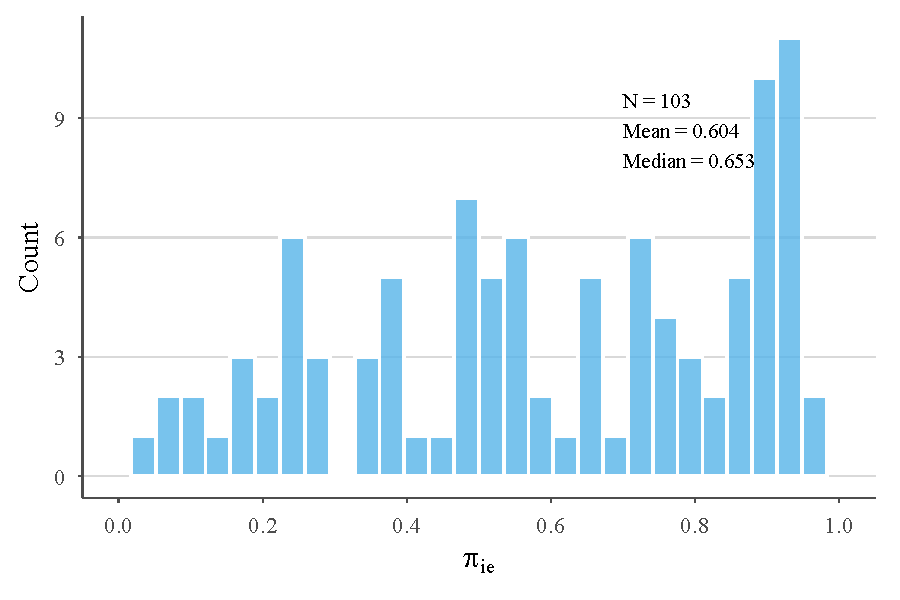
\includegraphics[width=0.48\textwidth]{../Figures/fig_pi_dist_gs.pdf}
\hfill
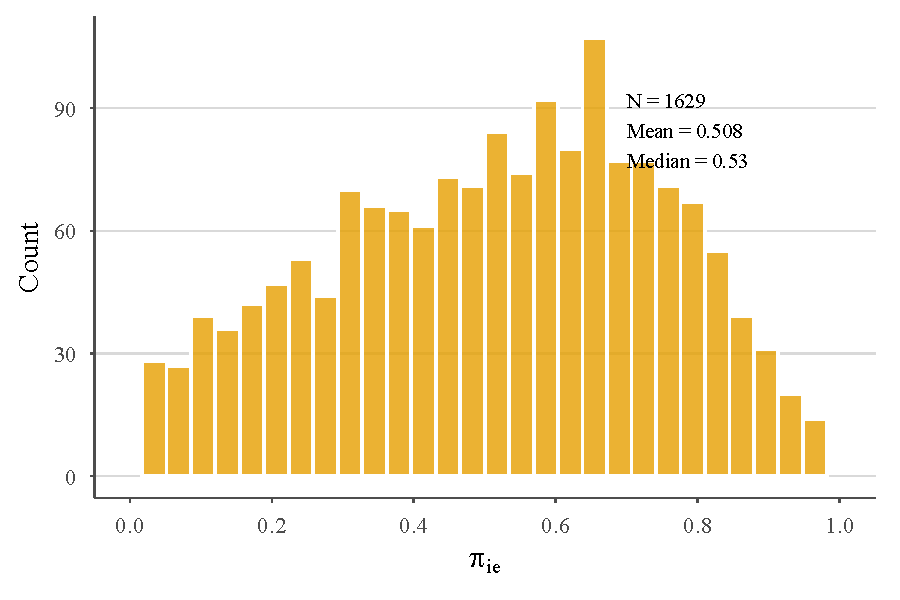
\includegraphics[width=0.48\textwidth]{../Figures/fig_pi_dist_nongs.pdf}
\caption{Distribution of Performance Probability $\pi_{ie}$ for LL Recipients}
\label{fig:pi_dist}
\begin{minipage}{0.9\textwidth}
\vspace{0.5em}
\footnotesize \textit{Notes.} Left panel: Grand Slam LL recipients. Right panel: non-Grand-Slam LL recipients. $\pi_{ie}$ is the product of match-level outcome probabilities from the match-winning logit. Lower values indicate more surprising tournament performances.
\end{minipage}
\end{figure}

\begin{table}[htbp]
\centering
\caption{Performance Probability Dose: Grand Slam (Stacked)}
\label{tab:perf_prob_gs}
\begin{threeparttable}
\small
\begin{tabular}{lccccc}
\toprule
 & 4w & 8w & 12w & 26w & 52w \\
\midrule
\multicolumn{6}{l}{\textit{Panel A: Matches won dose}} \\
\quad Ranking Points $\Delta$ (base) & 32.73 & 32.07 & -10.96 & -41.78 & -15.27 \\
 & (20.35) & (22.70) & (26.39) & (43.83) & (68.11) \\
\quad \quad $\times$ Matches Won & 33.46 & 83.80$^{**}$ & 76.60$^{*}$ & 144.52$^{**}$ & 221.02$^{**}$ \\
 & (36.78) & (40.37) & (40.77) & (55.32) & (106.99) \\[0.3em]
\quad Elo $\Delta$ (base) & 1.70 & -3.01 & -6.40 & 11.66 & 10.92 \\
 & (6.34) & (7.47) & (9.36) & (11.06) & (19.56) \\
\quad \quad $\times$ Matches Won & 13.94 & 22.52$^{*}$ & 27.06$^{*}$ & 23.61 & 24.79 \\
 & (10.81) & (12.40) & (13.93) & (15.03) & (23.36) \\[0.3em]
\quad Main Draws (base) & 0.34 & 0.56 & 0.53 & 0.64 & 0.04 \\
 & (0.34) & (0.37) & (0.40) & (0.55) & (1.37) \\
\quad \quad $\times$ Matches Won & -0.63 & -0.53 & -0.57 & 0.41 & 3.20$^{*}$ \\
 & (0.58) & (0.58) & (0.62) & (0.92) & (1.86) \\[0.3em]
\quad Matches (250+) (base) & 0.66 & 1.00$^{*}$ & 0.84 & 1.10 & -1.57 \\
 & (0.52) & (0.53) & (0.55) & (0.90) & (2.00) \\
\quad \quad $\times$ Matches Won & -1.06 & -0.26 & -0.30 & 1.24 & 7.75$^{**}$ \\
 & (1.02) & (0.96) & (1.00) & (1.32) & (3.11) \\[0.3em]
\quad Win \% (base) & 0.04 & -0.01 & -0.02 & -0.03 & 0.01 \\
 & (0.06) & (0.04) & (0.04) & (0.03) & (0.03) \\
\quad \quad $\times$ Matches Won & 0.06 & 0.06 & 0.05 & 0.05 & -0.00 \\
 & (0.09) & (0.06) & (0.05) & (0.04) & (0.04) \\[0.3em]
\\[0.5em]
\multicolumn{6}{l}{\textit{Panel B: Performance probability dose ($-\text{logit}(\pi)$)}} \\
\quad Ranking Points $\Delta$ (base) & 48.79$^{***}$ & 64.71$^{***}$ & 17.73 & 19.00 & 84.37 \\
 & (18.54) & (20.77) & (23.31) & (38.57) & (62.34) \\
\quad \quad $\times$ Dose & -2.47 & 5.86 & -1.92 & 24.84 & 47.63 \\
 & (13.59) & (16.53) & (16.94) & (22.74) & (43.90) \\[0.3em]
\quad Elo $\Delta$ (base) & 6.43 & 5.65 & 0.62 & 23.49$^{**}$ & 21.71 \\
 & (5.53) & (7.30) & (9.07) & (9.89) & (14.89) \\
\quad \quad $\times$ Dose & -2.88 & 2.10 & -3.20 & 8.03 & 2.81 \\
 & (3.87) & (4.61) & (5.12) & (5.88) & (10.12) \\[0.3em]
\quad Main Draws (base) & 0.08 & 0.30 & 0.24 & 0.75 & 1.19 \\
 & (0.31) & (0.33) & (0.34) & (0.52) & (1.18) \\
\quad \quad $\times$ Dose & -0.26 & -0.35$^{*}$ & -0.39$^{*}$ & -0.11 & 0.39 \\
 & (0.21) & (0.20) & (0.21) & (0.30) & (0.76) \\[0.3em]
\quad Matches (250+) (base) & 0.26 & 0.87$^{*}$ & 0.74 & 1.69$^{**}$ & 1.80 \\
 & (0.50) & (0.48) & (0.49) & (0.83) & (1.83) \\
\quad \quad $\times$ Dose & -0.41 & -0.35 & -0.25 & 0.30 & 2.41$^{**}$ \\
 & (0.39) & (0.33) & (0.36) & (0.50) & (1.21) \\[0.3em]
\quad Win \% (base) & 0.05 & 0.01 & -0.01 & -0.01 & 0.00 \\
 & (0.06) & (0.04) & (0.04) & (0.03) & (0.02) \\
\quad \quad $\times$ Dose & -0.03 & -0.02 & -0.03 & -0.01 & -0.02 \\
 & (0.04) & (0.02) & (0.02) & (0.01) & (0.01) \\[0.3em]
\midrule
$Z^{\text{pre}}$ controls & \multicolumn{5}{c}{Yes (horizon-interacted)} \\
\bottomrule
\end{tabular}

\begin{tablenotes}
\footnotesize
\item \textit{Notes.} Dose = $-\text{logit}(\pi_{ie})$ where $\pi_{ie}$ is the probability of observing the LL awardee's main-draw performance. Higher dose = more surprising performance. $^{***}p<0.01$, $^{**}p<0.05$, $^{*}p<0.10$.
\end{tablenotes}
\end{threeparttable}
\end{table}

\begin{table}[htbp]
\centering
\caption{Performance Probability Dose: Non-Grand-Slam (Stacked)}
\label{tab:perf_prob_nongs}
\begin{threeparttable}
\small
\begin{tabular}{lccccc}
\toprule
 & 4w & 8w & 12w & 26w & 52w \\
\midrule
\multicolumn{6}{l}{\textit{Panel A: Matches won dose}} \\
\quad Ranking Points $\Delta$ (base) & 12.91 & 4.34 & 2.78 & -12.83 & -15.81 \\
 & (9.93) & (10.69) & (11.61) & (17.59) & (34.82) \\
\quad \quad $\times$ Matches Won & 28.42$^{***}$ & 33.67$^{***}$ & 38.60$^{***}$ & 34.01$^{***}$ & 46.61 \\
 & (5.77) & (6.41) & (7.50) & (12.94) & (30.43) \\[0.3em]
\quad Elo $\Delta$ (base) & 4.40$^{*}$ & 4.08 & 7.09$^{**}$ & 3.34 & 2.86 \\
 & (2.65) & (2.88) & (3.05) & (4.83) & (6.68) \\
\quad \quad $\times$ Matches Won & 4.04$^{**}$ & 2.45 & 3.39 & 0.14 & -0.43 \\
 & (1.70) & (2.07) & (2.35) & (3.84) & (6.52) \\[0.3em]
\quad Main Draws (base) & -0.89$^{***}$ & -0.46$^{***}$ & -0.11 & 1.04$^{***}$ & 2.40$^{***}$ \\
 & (0.14) & (0.13) & (0.12) & (0.18) & (0.46) \\
\quad \quad $\times$ Matches Won & -0.06 & -0.03 & 0.06 & 0.34$^{**}$ & 1.58$^{***}$ \\
 & (0.10) & (0.09) & (0.10) & (0.17) & (0.46) \\[0.3em]
\quad Matches (250+) (base) & -1.73$^{***}$ & -1.09$^{***}$ & -0.55$^{**}$ & 1.60$^{***}$ & 4.66$^{***}$ \\
 & (0.29) & (0.26) & (0.25) & (0.38) & (0.91) \\
\quad \quad $\times$ Matches Won & -0.12 & 0.03 & 0.27 & 0.50 & 2.29$^{***}$ \\
 & (0.20) & (0.18) & (0.20) & (0.33) & (0.85) \\[0.3em]
\quad Win \% (base) & 0.02 & 0.02 & 0.01 & -0.00 & 0.00 \\
 & (0.02) & (0.01) & (0.01) & (0.01) & (0.01) \\
\quad \quad $\times$ Matches Won & -0.00 & -0.02 & -0.01 & -0.00 & -0.01 \\
 & (0.01) & (0.01) & (0.01) & (0.01) & (0.01) \\[0.3em]
\\[0.5em]
\multicolumn{6}{l}{\textit{Panel B: Performance probability dose ($-\text{logit}(\pi)$)}} \\
\quad Ranking Points $\Delta$ (base) & 28.46$^{***}$ & 23.10$^{**}$ & 23.60$^{**}$ & 4.46 & 6.48 \\
 & (9.50) & (10.20) & (11.30) & (15.62) & (31.01) \\
\quad \quad $\times$ Dose & 13.64$^{***}$ & 16.80$^{***}$ & 19.39$^{***}$ & 16.94$^{*}$ & 16.70 \\
 & (3.77) & (4.49) & (5.01) & (9.38) & (17.97) \\[0.3em]
\quad Elo $\Delta$ (base) & 6.56$^{***}$ & 5.34$^{*}$ & 8.75$^{***}$ & 2.98 & 1.32 \\
 & (2.54) & (2.76) & (2.93) & (4.37) & (5.94) \\
\quad \quad $\times$ Dose & 2.52$^{**}$ & 1.37 & 2.72 & 0.23 & -5.42 \\
 & (1.19) & (1.43) & (1.71) & (2.67) & (3.75) \\[0.3em]
\quad Main Draws (base) & -0.91$^{***}$ & -0.46$^{***}$ & -0.06 & 1.24$^{***}$ & 3.22$^{***}$ \\
 & (0.13) & (0.12) & (0.11) & (0.16) & (0.41) \\
\quad \quad $\times$ Dose & -0.02 & 0.01 & 0.06 & 0.24$^{**}$ & 0.88$^{***}$ \\
 & (0.07) & (0.06) & (0.07) & (0.11) & (0.30) \\[0.3em]
\quad Matches (250+) (base) & -1.78$^{***}$ & -1.06$^{***}$ & -0.39 & 1.89$^{***}$ & 5.86$^{***}$ \\
 & (0.26) & (0.25) & (0.24) & (0.36) & (0.81) \\
\quad \quad $\times$ Dose & -0.07 & 0.05 & 0.20 & 0.32 & 1.17$^{**}$ \\
 & (0.13) & (0.12) & (0.13) & (0.21) & (0.55) \\[0.3em]
\quad Win \% (base) & 0.02 & 0.01 & 0.00 & -0.00 & -0.01 \\
 & (0.02) & (0.01) & (0.01) & (0.01) & (0.01) \\
\quad \quad $\times$ Dose & 0.01 & 0.00 & 0.00 & 0.00 & 0.00 \\
 & (0.01) & (0.01) & (0.01) & (0.00) & (0.00) \\[0.3em]
\midrule
$Z^{\text{pre}}$ controls & \multicolumn{5}{c}{Yes (main effects)} \\
\bottomrule
\end{tabular}

\begin{tablenotes}
\footnotesize
\item \textit{Notes.} Same specification as Table~\ref{tab:perf_prob_gs} with control function correction. $^{***}p<0.01$, $^{**}p<0.05$, $^{*}p<0.10$.
\end{tablenotes}
\end{threeparttable}
\end{table}

\subsection{Non-Grand-Slam Extension}
\label{sec:results_nongs}

The non-Grand-Slam control function estimates, which draw on the larger ATP sample ($N = 2{,}708$, with 874 treated) and the WTA sample ($N = 2{,}545$, with 755 treated), provide corroborating evidence. The generalized residual $\hat{v}_{ie}$ from the corrected selection probability $P_i^{LL}$---computed via exact enumeration of the full combinatorial structure of qualifying match pairings---enters all non-GS specifications to account for endogenous LL assignment.

\paragraph{ATP non-GS results.} Ranking point gains are 12.2 at 4 weeks ($p = 0.065$), 11.0 at 8 weeks ($p = 0.127$), and 28.1 at 26 weeks ($p = 0.009$), fading to 6.5 at 52 weeks ($p = 0.776$). Tournament access effects emerge at longer horizons: main draw entries increase by 1.7 at 26 weeks ($p < 0.001$) and 5.0 at 52 weeks ($p < 0.001$), and matches at 250+ events increase by 2.8 at 26 weeks ($p < 0.001$) and 8.6 at 52 weeks ($p < 0.001$). Elo effects are null at all horizons. The endogeneity test (coefficient on $\hat{v}_{ie}$) is insignificant for ranking point outcomes (all $p > 0.10$), suggesting that OLS would be consistent for this outcome. However, $\hat{\rho}$ is significant for tournament access outcomes---main draws entered and matches at 250+ events---at short and long horizons ($p < 0.01$), confirming that the control function correction is necessary for count-based outcomes.

\paragraph{WTA non-GS results.} The WTA non-Grand-Slam sample yields a ranking point gain of 27.4 at 4 weeks ($p = 0.004$) and 22.2 at 8 weeks ($p = 0.028$), with the effect persisting at 12 weeks (23.0, $p = 0.042$) before fading at 26 weeks (3.1, $p = 0.842$). The WTA access outcomes at 26 weeks are significant---main draw entries ($+1.2$, $p < 0.001$) and matches at 250+ events ($+1.9$, $p < 0.001$). The WTA non-GS Elo results differ from the Grand Slam pattern: Elo gains are significant at 4 weeks (6.6, $p = 0.008$), 8 weeks (5.5, $p = 0.050$), and 12 weeks (8.9, $p = 0.002$), fading at longer horizons. This short-horizon Elo effect on the WTA tour is consistent with the marginally significant WTA GS Elo result ($p = 0.070$ at 4 weeks), though the match-level tournament performance model (Section~\ref{sec:mechanisms_performance}) finds no significant effect on win probability conditional on opponent strength on either tour. The WTA Elo gains at short horizons may reflect favorable opponent draws in additional tournaments rather than improved competitive skill per se.

The non-Grand-Slam CF estimates are broadly consistent with the Grand Slam lottery in direction and magnitude. The ATP CF finds ranking point gains of 28.1 points at 26 weeks ($p = 0.009$), compared to 49.2 points from the GS lottery ($p = 0.054$). Tournament access effects are directionally consistent: the CF finds 1.7 additional main draws at 26 weeks ($p < 0.001$), compared to 1.1 from the GS lottery ($p = 0.006$). The WTA non-GS results show stronger and more persistent short-horizon effects than the earlier estimates, with significant ranking point gains through 12 weeks and significant Elo gains through 12 weeks.

Full non-Grand-Slam tables are reported in the appendix: the ATP CF dynamics (Table~\ref{tab:dynamic_nongs_iv}), WTA CF dynamics (Table~\ref{tab:dynamic_nongs_wta}), heterogeneity (Tables~\ref{tab:hetero_nongs} and~\ref{tab:hetero_nongs_wta}), first-LL results (Tables~\ref{tab:firstll_nongs} and~\ref{tab:firstll_nongs_wta}), and the LL distribution (Table~\ref{tab:ll_dist_nongs}).
